\chapter{Related Work}\label{Related_Work}
In this section of the bachelor thesis, related works are addressed. Firstly, reference will be made to similar projects where instances were created using the \textsc{Cinco} Meta Modeling Tool. This is followed by scholarly works that provide more information on MDSD and SCCharts.
\section{Modeling with \textsc{Cinco} related}
For a better understanding of the background of \textsc{Cinco} and the reasons for its development, paper~\cite{Naujokat.2018} provides a comprehensive overview. In addition to the topics mentioned earlier, it also suggests application areas and compares the tool with other meta-modeling tools. Furthermore, it offers a guide on how to create DSLs with \textsc{Cinco}.

In "A Tutorial Introduction to Graphical Modeling and Metamodeling with \textsc{Cinco}" by Lybecait et al.~\cite{Lybecait.2018} presented a \textsc{Cinco} Project that can be used to create web stories, an adventure game. The primary goal was to showcase the two recent additions, Pyro and GCS (Graphical \textsc{Cinco} Specification): Pyro extends the \textsc{Cinco} ecosystem by enabling web-based modeling for \textsc{Cinco}-based graphical modeling languages, while GCS introduces graphical editors to the meta-level in a bootstrapping fashion. This is aimed at reducing the complexity of creating DSLs via \textsc{Cinco} and improving the overall process. The Project can be found here under examples~\cite{.06.05.2022}. 

The second project is a graphical language for statecharts, similar to the one designed in this bachelor thesis. However, instead of using a code generator, an additional simulator for the input was implemented. A screenshot of it can be seen in Figure \ref{fig:CINCO_Statechart_Example} While there is no written thesis available, this project is well-suited for exploring the features of \textsc{Cinco}. It can also be found at~\cite{.06.05.2022} under examples.
\begin{figure}[h!]
\centering
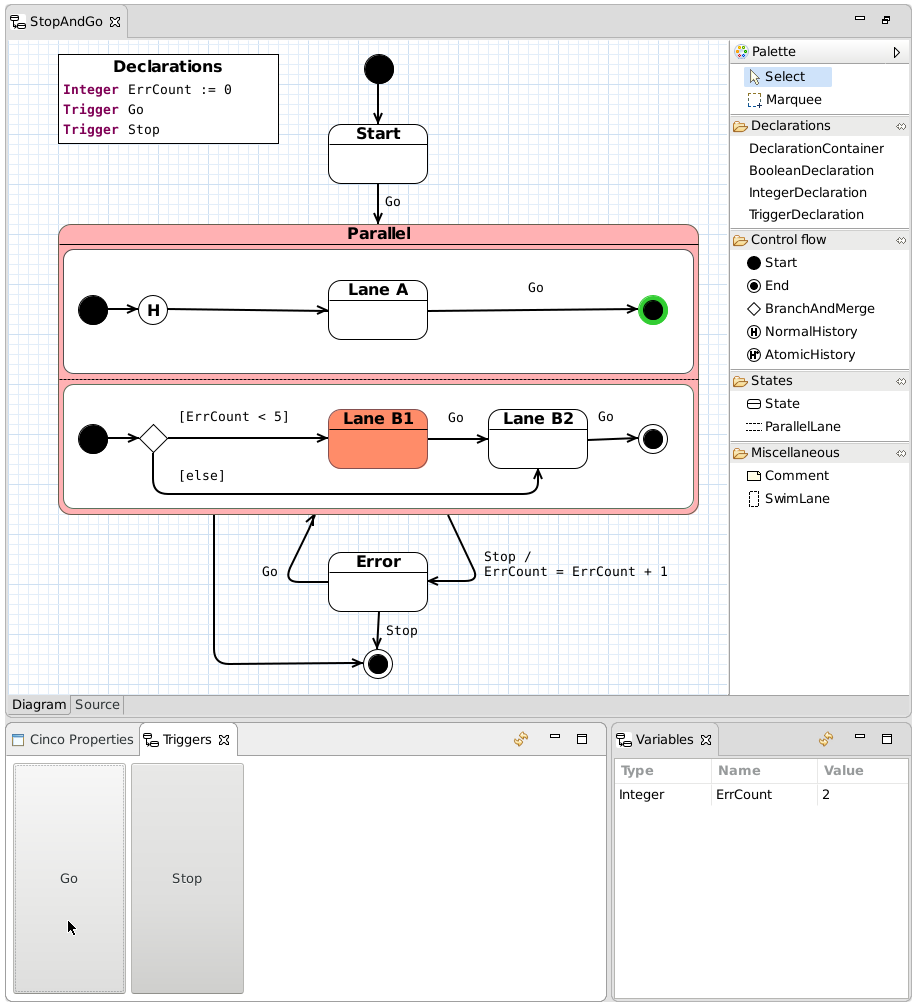
\includegraphics[width=0.8\textwidth]{bilder/CINCO_Statechart_Example}
\caption{StateChart Model and Simulation Screenshot of the \textsc{Cinco} Statechart Project~\cite{.06.05.2022}.}
\label{fig:CINCO_Statechart_Example}
\end{figure} 
\section{Model-Driven-Software Engineering related}
For a very detailed introduction to the topic of Model-Driven Software Engineering, the book by Brambilla, Cabot and Wimmer "MODEL-DRIVEN SOFTWARE ENGINEERING IN PRACTICE"~\cite{Brambilla.2017}, which is often used as a reference here, is highly recommended. In the first section, the authors delve into the basics of MDSE, its use cases, and how to integrate MDSE into existing development processes. In the second section, they delve further into the technical aspects, such as creating a domain-specific modeling language and designing functions for model-to-model and model-to-text transformations.
\section{Sequentially Constructive Statecharts related}
SCCharts have been briefly discussed here to provide a broad overview of this visual language. Some aspects have only been touched upon lightly or not covered extensively to avoid exceeding the scope of this work. For a comprehensive explanation of the SCCharts language and its suitability for implementing safety-critical systems, please refer to Motika's dissertation titled "SCCharts - Language and Interactive Incremental Compilation"~\cite{Motika.2017}. In this source, also detailed explanations of additional features can be found, such as the integration of host code or the pre() operator.